%%%%%%%%%%%%%%%%%%%%%%%%%%%%%%%%%%%%%%%%%%%%%%%%%%%%%%%%%%%%%%%%%%%%%%%%%%%%
% AGUtmpl.tex: this template file is for articles formatted with LaTeX2e,
% Modified March 2009
%
% This template includes commands and instructions
% given in the order necessary to produce a final output that will
% satisfy AGU requirements.
%
% PLEASE DO NOT USE YOUR OWN MACROS
%
% For more information on using the AGUTeX macro package,
% see agudocs.tex or agudocs.pdf
%
%%%%%%%%%%%%%%%%%%%%%%%%%%%%%%%%%%%%%%%%%%%%%%%%%%%%%%%%%%%%%%%%%%%%%%%%%%%%
%
% All questions should be e-mailed to author.help@agu.org.
%
%%%%%%%%%%%%%%%%%%%%%%%%%%%%%%%%%%%%%%%%%%%%%%%%%%%%%%%%%%%%%%%%%%%%%%%%%%%%
%
% Step 1: set the \documentclass
%
% The three options for article format are: two-column (default),
% draft, for initial article submission; and galley for narrow
% single columns.
%
% PLEASE USE THE DRAFT OPTION TO SUBMIT YOUR PAPERS
% The draft option produces double spaced output
%
% Choose the journal abbreviation for the journal you are
% submitting to:

% jgrga JOURNAL OF GEOPHYSICAL RESEARCH
% gbc   GLOBAL BIOCHEMICAL CYCLES
% grl   GEOPHYSICAL RESEARCH LETTERS
% pal   PALEOCEANOGRAPHY
% ras   RADIO SCIENCE
% rog   REVIEWS OF GEOPHYSICS
% tec   TECTONICS
% wrr   WATER RESOURCES RESEARCH
% gc    GEOCHEMISTRY, GEOPHYSICS, GEOSYSTEMS

% (If you are submitting to a journal other than jgrga,
% substitute the initials of the journal for "jgrga" below)

\documentclass[draft,grl]{agutex}

%%%%%%%%%%%%%%%%%%%%%%%%%%%%%%%%%%%%%%%%%%%%%%%%%%%%%%%%%%
%%%% optional article formats author might want to use

% To produce a galley version:
% \documentclass[galley,jgrga]{AGUTeX}

% To produce a two columned version:
% \documentclass[jgrga]{AGUTeX}

%%%%%%%%%%%%%%%%%%%%%%%%%%%%%%%%%%%%%%%%%%%%%%%%%%%%%%%%%%%%%%%%%%%%%%%%%
% OPTIONAL:
% To print your article using PostScript fonts, uncomment this:
% \usepackage{agu-ps}
% You many need to edit the top of agu-ps to use the names of the PS
% fonts on your system.

%%%%%%%%%%%%%%%%%%%%%%%%%%%%%%%%%%%%%%%%%%%%%%%%%%%%%%%%%%%%%%%%%%%%%%%%%
% OPTIONAL:
% To Create numbered lines:

% If you don't already have lineno.sty, you can download it from
% http://www.ctan.org/tex-archive/macros/latex/contrib/ednotes/
% (or google lineno.sty ctan), available at TeX Archive Network (CTAN).
% Take care that you always use the latest version.

% To activate the commands, uncomment \usepackage{lineno}
% and \linenumbers*[1]command, below:

\usepackage{lineno}
\linenumbers*[1]

%%%%%%%%%%%%%%%%%%%%%%%%%%%%%%%%%%%%%%%%%%%%%%%%%%%%%%%%%%%%%%%%%%%%%%%%%
% Figures and Tables
%

% When submitting articles through the GEMS system:
% COMMENT OUT ANY COMMANDS THAT INCLUDE GRAPHICS.
% (See FIGURES section near the end of the file)


%  Figures and Tables should be placed at the end of the article,
%  after the references.
%
%  Uncomment the following command to include .eps files
%  (comment out this line for draft format):
\usepackage[dvips]{graphicx}
%
%    Uncomment the following command to allow illustrations to print
%    when using Draft:
\setkeys{Gin}{draft=false}
%
% Substitute one of the following for [dvips] above
% if you are using a different driver program and want to
% proof your illustrations on your machine:
%
% [xdvi], [dvipdf], [dvipsone], [dviwindo], [emtex], [dviwin],
% [pctexps],  [pctexwin],  [pctexhp],  [pctex32], [truetex], [tcidvi],
% [oztex], [textures]
%
% See how to enter figures and tables at the end of the article, after
% references.
%
%% ------------------------------------------------------------------------ %%
%
%  ENTER PREAMBLE
%
%% ------------------------------------------------------------------------ %%

% Author names in capital letters:
\authorrunninghead{DAWE AND AUSTIN}

% Shorter version of title entered in capital letters:
\titlerunninghead{RECONCILING LES ENTRAINMENT}

% Author mailing address: please repeat this command for
% each author and alphabetize authors:

\authoraddr{Philip H. Austin,
Department of Earth and Ocean Sciences, University of
British Columbia, 6339 Stores Road, Vancouver, BC, V6T 1Z4, Canada.
(paustin@eos.ubc.ca)}

\authoraddr{Jordan T. Dawe,
Department of Earth and Ocean Sciences, University of
British Columbia, 6339 Stores Road, Vancouver, BC, V6T 1Z4, Canada.
(jdawe@eos.ubc.ca)}

\begin{document}

%% ------------------------------------------------------------------------ %%
%
%  TITLE
%
%% ------------------------------------------------------------------------ %%


\title{Reconciling direct and bulk tracer measurements of LES cloud entrainment}
%

%% ------------------------------------------------------------------------ %%
%
%  AUTHORS AND AFFILIATIONS
%
%% ------------------------------------------------------------------------ %%


%Use \author{\altaffilmark{}} and \altaffiltext{}

% \altaffilmark will produce footnote;
% matching altaffiltext will appear at bottom of page.
% May use \\ to start a new line.

\authors{Jordan T. Dawe\altaffilmark{1} and Philip H. Austin\altaffilmark{1}}

\altaffiltext{1}{Department of Earth and Ocean Sciences, 
                      University of British Columbia, Vancouver, BC, Canada}

%% ------------------------------------------------------------------------ %%
%
%  ABSTRACT
%
%% ------------------------------------------------------------------------ %%

% >> Do NOT include any \begin...\end commands within
% >> the body of the abstract.

\begin{abstract}
Direct measurements of entrainment and detrainment rates from LES model 
cloud fields produce values twice as large as those produced from bulk 
conserved tracer budget calculations.  This discrepancy is partly the 
result of numerical errors, but mostly due to neglect of the influence of 
the moistened cloud environment on the tracer budget calculations.  
Correcting the entrainment and detrainment values to account for the effect 
of the shell of moist air around the clouds corrects this over-estimate.  
\end{abstract}

%% ------------------------------------------------------------------------ %%
%
%  BEGIN ARTICLE
%
%% ------------------------------------------------------------------------ %%

% The body of the article must start with a \begin{article} command
%
% \end{article} must follow the references section, before the figures
%  and tables.

\begin{article}

%% ------------------------------------------------------------------------ %%
%
%  TEXT
%
%% ------------------------------------------------------------------------ %%

\section{Introduction}

The rate at which air is entrained into and detrained from clouds is a major 
control on cloud properties, cloud top height, and the amount of heat and 
moisture clouds transport upward.  As such, proper simulation of the 
subgrid-scale effects of cumulus clouds in General Circulation Models (GCMs) 
requires understanding cloud entrainment and detrainment.

Large Eddy Simulation (LES) is a primary tool used to studying cloud mass
exchange dynamics.  LES entrainment and detrainment rates are typically 
calculated by recording budgets of bulk conserved tracer variables and 
inferring the amount of fluid exchange between the clouds and the surrounding 
air that is needed to balance vertical advection rates within the cloud field 
\citep{Siebesma1995}.

Alternatively, entrainment and detrainment can simply be calculated directly 
from the LES velocity and tracer fields.  \cite{Romps2010} recently presented 
a technique to directly measure entrainment and detrainment in this manner, 
and found that direct measurement produced values roughly twice as large as 
tracer budget calculations.  Romps attributed this difference to the assumption 
made in bulk tracer calculations that the fluid exchanged between clouds and 
environment had the mean properties of the cloud or environment, respectively.

Here we examine the sources of this factor of two discrepancy.  We show the 
discrepancy can be explained by three effects: the presence of a moist shell 
of recently detrained air surrounding the clouds, Reynolds correlations 
between the entrainment rates and the cloud bulk tracer values, and 
inconsistancies in the numerical methods used in the two calculations.

%===================================================

\section{Model desccription}

All calculations in this paper were made using the System for Atmospheric 
Modeling \citep[SAM;][]{Khairoutdinov2003}, run with a standard GCSS Barbados 
Oceanographic and Meteorological Experiment (BOMEX) LES simulation 
\citep{Holland1973, Siebesma2003}.  The model was run on a 6.4 km x 6.4 km 
horizontal x 3.2 km vertical domain at 25 meter grid resolution in all 
directions.  The model was run for 6 hours, and the first three hours 
of simulation were discarded; 15 minute averages were output for the terms 
in each of our calculations.  

We have implemented the direct entrainment calculation scheme of 
\cite{Romps2010} and a direct entrainment method of our own devising 
\citep{Dawe2011} in SAM and use these methods for the calculation of direct flux 
values of entrainment and detrainment.

\section{Correction of direct flux calculations}

\cite{Siebesma1995} derive equations for entrainment and detrainment from a 
simple entraining cloud plume based on conserved bulk tracer properties:
\begin{equation}
  \label{eq:siebesma_entrainment}
    E_{\chi}(\chi_c - \chi_e) = - M_c \frac{\partial \chi_c}{\partial z}
        - \frac{\partial \rho a \overline{w' \chi'}^c}{\partial z}
        - \rho a \frac{\partial \chi_c}{\partial t}
        + a \rho \left(\frac{\partial \bar{\chi}}{\partial t}\right)_{forcing}
\end{equation}
and
\begin{equation}
  \label{eq:siebesma_detrainment}
    D_{\chi}(\chi_c - \chi_e) = - M_c \frac{\partial \chi_e}{\partial z}
        + \frac{\partial \rho (1 - a) \overline{w' \chi'}^e}{\partial z}
        + \rho (1-a) \frac{\partial \chi_e}{\partial t}
     - \rho (1-a) \left(\frac{\partial \bar{\chi}}{\partial t}\right)_{forcing}
\end{equation}
Here $\chi$ represents any conserved bulk tracer, such as $q_t$ or $h$; $a$ is 
the fractional cloud core area; $M_c$ is vertical cloud core mass flux 
(kg m$^{-2}$ s$^{-1}$); $w$ is vertical velocity (m s$^{-1}$); $\rho$ is the 
density of the air in kg m$^{-3}$; $e$ and $c$ sub- and super-scripts denote 
horizontally averaged values conditionally sampled in the cloud environment and 
core; $forcing$ refers to forcings not included in the other terms, such as 
radiation or subsidence; primed values represent anomalies relative to the 
horizontal mean; overbars represent horizontal averaging; and $E_{\chi}$ and 
$D_{\chi}$ are the horizontally averaged bulk tracer entrainment into and 
detrainment out of the cloud core in kg s$^{-1}$ m$^{-3}$.  Cloud core is 
defined here as model points that have condensed water, upward vertical 
velocity, and are positively buoyant relative to the horizontal mean.  
Equations (\ref{eq:siebesma_entrainment}) and (\ref{eq:siebesma_detrainment}) 
are essentially tracer budgets which balance vertical fluxes and time 
tendencies of conserved tracers in the clouds against horizontal exchanges.

Equations (\ref{eq:siebesma_entrainment}) and (\ref{eq:siebesma_detrainment}) 
have one obvious source of bias: the assumption that all fluid entrained or 
detrained from the cloud has the mean properties of the environment or cloud, 
respectively.  Examination of the cloud core edge properties (defined as cloud 
core model grid cells that are horizontally adjacent to non-core cells) shows 
the cloud core edge has nearly the same properties as the mean core, while the 
cloud core shell properties (non-core cells that are horizontally adjacent to 
core cells) are significantly different than mean environment properties 
(Figure \ref{fig:shell_correction}a).  This is in agreement with previous 
results from both LES modeling and observations \citep{Heus2008}.
  
Here we derive a correction to equations (\ref{eq:siebesma_entrainment}) and 
(\ref{eq:siebesma_detrainment}) to account for the presence of this the moist 
cloud shell and dry cloud edge.  We start our derivation by modifying equation 
(5.1) from \cite{Siebesma1995}, replacing the mean cloud core and environment 
values of the bulk tracers in the entrainment and detrainment terms with the 
edge and shell properties:
\begin{eqnarray}
  \label{eq:entrainment_derivation_1}
    \rho \frac{\partial a \chi_c}{\partial t} 
    = - \frac{\partial M_c \chi_c}{\partial z} 
    + E_d \chi_{se} - D_d \chi_{sc} 
    - \frac{\partial \rho a \overline{w' \chi'}^c}{\partial z} 
    + a \rho \left(\frac{\partial \bar{\chi}}{\partial t}\right)_{forcing}
\end{eqnarray}
\begin{eqnarray}
  \label{eq:detrainment_derivation_1}
    \rho \frac{\partial (1 - a) \chi_e}{\partial t}
    = \frac{\partial M_c \chi_e}{\partial z} 
    - E_d \chi_{se} + D_d \chi_{sc} 
    - \frac{\partial \rho (1 - a) \overline{w' \chi'}^e}{\partial z} 
    + \rho (1 - a) \left(\frac{\partial \bar{\chi}}{\partial t}\right)_{forcing}
\end{eqnarray}
here we have replaced $\chi_e$ in the entrainment term with $\chi_{se}$, the 
bulk tracer value immediately outside the cloud surface (the "cloud shell"), and 
$\chi_c$ in the detrainment term with $\chi_{sc}$, the bulk tracer value 
immediately inside the cloud surface (the "cloud edge").  $E_d$ and $D_d$ are 
the direct mass flux values of the entrainment and detrainment, in kg s$^{-1}$ 
m$^{-3}$.

Next we substitute in the continuity equation for a cloud plume,
\begin{equation}
   \label{eq:continuity}
   \rho \frac{\partial a}{\partial t} 
   + \frac{\partial M_c}{\partial z} = E_d - D_d
\end{equation}
This allows us to write:
\begin{eqnarray}
  \label{eq:entrainment_derivation_2}
    E_d (\chi_{se} - \chi_c) + D_d (\chi_c - \chi_{sc}) 
    = M_c \frac{\partial \chi_c}{\partial z}
    + \frac{\partial \rho a \overline{w' \chi'}^c}{\partial z} 
    + \rho a \frac{\partial \chi_c}{\partial t}
    - a \rho \left(\frac{\partial \bar{\chi}}{\partial t}\right)_{forcing}
\end{eqnarray}
\begin{eqnarray}
  \label{eq:detrainment_derivation_2}
    D_d (\chi_e - \chi_{sc}) + E_d (\chi_{se} - \chi_e)
    = M_c \frac{\partial \chi_e}{\partial z}
    - \frac{\partial \rho (1 - a) \overline{w' \chi'}^e}{\partial z} 
    - \rho (1 - a) \frac{\partial \chi_e}{\partial t}
    + \rho (1 - a) \left(\frac{\partial \bar{\chi}}{\partial t}\right)_{forcing}
\end{eqnarray}

Finally, we substitute in equations (\ref{eq:siebesma_entrainment}) and 
(\ref{eq:siebesma_detrainment}) for the bulk tracer tendency terms and 
rearrange to get:
\begin{equation}
  \label{eq:corrected_entrainment}
    E_{\chi} = \frac{(\chi_{c} - \chi_{se})E_d - (\chi_{c} - \chi_{sc})D_d}
             {(\chi_{c} - \chi_{e})}
\end{equation}
\begin{equation}
  \label{eq:corrected_detrainment}
    D_{\chi} = \frac{(\chi_{sc} - \chi_{e})D_d - (\chi_{se} - \chi_{e})E_d}
             {(\chi_{c} - \chi_{e})}
\end{equation}

Note that under this correction $E_d-D_d = E_{\chi}-D_{\chi}$, preserving 
mass continuity.

We can immediately see this correction has two effects.  First, it reduces
the direct entrainment by a factor of
$(\chi_{c} - \chi_{se})/(\chi_{c} - \chi_{e})$ and the direct detrainment 
by a factor of $(\chi_{sc} - \chi_{e})/(\chi_{c} - \chi_{e})$, to account for 
the smaller amount of mean cloud or environment air needed to balance the 
bulk tracer tendency terms relative to edge or shell air.  Second, the 
correction also reduces the direct entrainment by 
$D_d(\chi_{c} - \chi_{sc})/(\chi_{c} - \chi_{e})$ and the direct detrainment 
by $E_d(\chi_{se} - \chi_{e})/(\chi_{c} - \chi_{e})$, to account for changes 
in the mean core and environment bulk tracer budgets due to entraining 
parcels moister than the environmental mean and detraining parcels dryer than 
the cloud mean.  

Comparison of the values inferred from bulk tracer budget calculations with 
direct flux values calculated by the method of \cite{Romps2010} shows the 
direct flux values are significantly larger than the bulk tracer values 
(Figure \ref{fig:shell_correction}, b and c).  Correcting the direct flux 
entrainment and detrainment values using equations 
(\ref{eq:corrected_entrainment}) and (\ref{eq:corrected_detrainment}) results 
in much better agreement with the bulk tracer calculations.  Relative to the 
bulk tracer calculation, the corrected values are still too large near cloud 
base and too small above cloud base; however, the correction does duplicate the 
negative detrainment values near cloud base that are typically produced by bulk 
tracer calculations.

%==============================================================================

\section{Correcting for Reynolds correlations}

Using the mean values of the cloud core edge and shell neglects the possibility 
of Reynolds correlations between the entrainment or detrainment and the total 
specific water values.  These can be evaluated using relations derived by 
\cite{Romps2010}.  First, Romps defines the direct flux entrainment and 
detrainment as:
\begin{equation}
  \label{eq:romps_e_minus_d}
  e - d = \frac{\partial}{\partial t}(A\rho) 
        + \nabla \cdot (\rho \mathbf{u} A) 
\end{equation}
Here $e$ and $d$ are the local entrainment and detrainment through the cloud 
surface in kg s$^{-1}$ m$^{-3}$, $\mathbf{u}$ is the velocity of the air in 
m s$^{-1}$, and $A$ is the "activity" of the fluid, where $A$ is one at "active" 
cloud core points and zero otherwise.  The values of $e - d$ are averaged 
over the length of time a grid cell experiences mass fluxes between an active 
and an inactive point; positive $e-d$ values are then considered to be purely 
$e$ and negative values, $d$.  Note that $E_d = \overline{e}$ and 
$D_d = \overline{d}$.

Next, Romps define the tracer flux to be:
\begin{equation}
  \label{eq:romps_echi_minus_dchi}
  e\chi - d\chi = \frac{\partial}{\partial t}(\chi A \rho) 
                + \nabla \cdot (\chi \rho \mathbf{u} A) 
\end{equation}
where $\chi$ is the local value of the bulk conserved tracer, and the same time 
averaging applies as in equation (\ref{eq:romps_e_minus_d}).  Using these two 
calculations we can define the effective tracer value of entraining parcels to 
be:
\begin{equation}
  \label{eq:chi_re}
  \chi_{re} = \frac{\overline{e\chi} }{E_d} 
            = \chi_{se} + \frac{\overline{e' \chi'}}{E_d}
\end{equation}
and of detraining parcels to be:
\begin{equation}
  \label{eq:chi_rc}
  \chi_{rc} = \frac{\overline{d\chi}}{D_d} 
            = \chi_{sc} + \frac{\overline{d' \chi'}}{D_d}
\end{equation}
Thus, we can see the mean cloud edge and shell values should be modified by 
the Reynolds correlations between entrainment and tracer values.

The values of $\chi_{rc}$ and $\chi_{re}$ show significant deviations from 
the mean edge and shell values (Figure \ref{fig:Reynolds_correction}a).
In general, the inclusion of Reynolds correlations decreases the effective 
shell and core tracer values, indicating $q_t$ and $e$ or $d$ are typically 
anti-correlated; more entrainment and detrainment occurs when $q_t$ values are 
low, and less when $q_t$ values are high.  Applying these effective cloud edge 
and shell $q_t$ values to equations (\ref{eq:corrected_entrainment}) and 
(\ref{eq:corrected_detrainment}) results in much better agreement with the bulk 
tracer calculations than simply using the mean edge and shell values 
(Figure \ref{fig:Reynolds_correction}b and c).  However, a small discrepancy 
still remains to be explained.

%==============================================================================

\section{Comparison of Siebesma and Romps bulk tracer calculations}

\cite{Romps2010} derives alternate equations equivalent to 
(\ref{eq:siebesma_entrainment}) and (\ref{eq:siebesma_detrainment}) which use
direct tracer flux calculations in place of horizontally averaged tracer 
budgets.  \cite{Romps2010} derives tracer entrainment and detrainment to be:
\begin{equation}
  \label{eq:romps_entrainment}
  E_{\chi}(\chi_{c} - \chi_{e}) = \chi_{c}(E_d-D_d) 
                                - (\overline{e\chi} - \overline{d\chi})
\end{equation}
\begin{equation}
  \label{eq:romps_detrainment}
  D_{\chi}(\chi_{c} - \chi_{e}) = \chi_{e}(E_d-D_d) 
                                - (\overline{e\chi} - \overline{d\chi})
\end{equation}

Expansion of these equations with (\ref{eq:romps_e_minus_d}) and 
(\ref{eq:romps_echi_minus_dchi}) and applying suitable averaging shows these 
equations to be formally identical to (\ref{eq:siebesma_entrainment}) and 
(\ref{eq:siebesma_detrainment}).  Despite this, these two methods of 
calculating $E_{\chi}$ and $D_{\chi}$ show average differences of 10-20\%
(Figure \ref{fig:numerical_correction}).  However, the direct flux entrainment 
and detrainment, corrected using the effective cloud edge and shell values 
including the effect of Reyonolds correlations, agrees exactly with the Romps
bulk tracer calculation.

We attribute these differences to numerical errors introduced by the 
different discretization schemes used in each calculation.  For instance, 
vertical gradients in the Siebesma method were calculated by finding 
horizontally averaged profiles of model quantities, then taking centered 
differences, while evaluating the divergence of $\chi \rho \mathbf{u} A$ in 
the Romps calculation was done using SAM's much more elaborate MPDATA tracer 
advection routine.  Since the Romps method of calculating $E_{\chi}$ and 
$D_{\chi}$ is more consistent with SAM's numerics, we take this to be the 
better representation of the bulk tracer calculation, and conclude that 
bulk tracer calculations using the methods of \cite{Siebesma1995} likely 
overestimate the true value by 10-20\%.

%==============================================================================

\section{Discussion and Conclusion}

We have shown it is possible to explain the differences between entrainment and 
detrainment values calculated via bulk tracer budgets and direct flux 
calculations by taking into account the properties of the cloud shell, the 
effect of Reynolds correlations between fluxes and tracer values, and 
accuracy differences in the numerical methods used by the two calculations.
This suggests that the presence of the moist cloud shell, and indeed the 
variability within this shell, has a significant role in mediating fluxes 
between the clouds and the environment, and may be an important factor in 
improving parameterizations of shallow convection.

We can also conclude that the bulk tracer calculations given by 
\cite{Siebesma1995} do not calculate the true mass fluxes that occur between 
cloud and environment.  To calculate the actual mass fluxes the bulk tracer 
equations must at least be corrected for the effect of the moist shell of 
evaporated air around the cloud.

Whether one cosiders the bulk tracer or direct flux values to be "correct" will 
depend on the purpose for which they are used.  The bulk tracer entrainment and 
detrainment values are more suited to calculating cloud moisture and energy 
fluxes in GCM parameterizations, which only have access to large-scale mean 
bulk tracer values.  On the other hand, the direct fluxes may be important for 
calculating fluxes of properties that have different radial dependencies than 
$q_t$ or $h$, such as vertical momentum, which is negative in the shell 
\citep{Heus2008}, or for aerosols whose chemical properties are altered by 
reactions in the presence of liquid water \citep{Hoppel1994}.  

%%% End of body of article:

%%%%%%%%%%%%%%%%%%%%%%%%%%%%%%%%
%% Optional Appendix goes here
%
%%%%%%%%%%%%%%%%%
% Geophysical Research Letters only allows an appendix without a letter.
%% You can get this result with
%  \section*{Appendix}
%  or
%  \section*{Appendix: Title}
%%%%%%%%%%%%%%%%%
%
% \appendix resets counters and redefines section heads
% but doesn't print anything.
% After typing  \appendix
%
% \section{Here Is Appendix Title}
% will print
% Appendix A: Here Is Appendix Title
%
% \section*{Appendix}
% will print
% Appendix
%
% \section*{Appendix: Here Is Appendix Title}
% will print
% Appendix: Here Is Appendix Title
%
% For only 1 appendix \appendix \section{Appendix} is preferred.
% which will print
% Appendix A

%%%%%%%%%%%%%%%%%%%%%%%%%%%%%%%%%%%%%%%%%%%%%%%%%%%%%%%%%%%%%%%%
%
% Optional Glossary or Notation section, goes here
%
%%%%%%%%%%%%%%
% Glossary only allowed in Reviews of Geophysics
% \section*{Glossary}
% \paragraph{Term}
% Term Definition here
%
%%%%%%%%%%%%%%
% Notation -- End each entry with a period.
% \begin{notation}
% Term & definition.\\
% Second Term & second definition.
% \end{notation}
%%%%%%%%%%%%%%%%%%%%%%%%%%%%%%%%%%%%%%%%%%%%%%%%%%%%%%%%%%%%%%%%
%
%  ACKNOWLEDGMENTS

\begin{acknowledgments}
Support for this work was provided by the Canadian Foundation for Climate and 
Atmospheric Science through the Cloud Aerosol Feedback and Climate network.
All figures were generated using the matplotlib library in the Python
programming language.
\end{acknowledgments}

%% ------------------------------------------------------------------------ %%
%
%  REFERENCE LIST AND TEXT CITATIONS
%
% Either type in your references using
% \begin{thebibliography}{}
% \bibitem{}
% Text
% \end{thebibliography}
%
% Or,
%
% If you use BiBTeX for your References, please produce your .bbl
% file and copy the contents into your paper here.
%
% Follow these steps:
% 1. Run LaTeX on your LaTeX file.
%
% 2. Run BiBTeX on your LaTeX file.
%
% 3. Open the new .bbl file containing the reference list and
%   copy all the contents into your LaTeX file here.
%
% 4. Comment out the old \bibliographystyle and \bibliography commands.
%
% 5. Run LaTeX on your new file before submitting.
%
% AGU does not want a .bib or a .bbl file, but asks that you
% copy in the contents of your .bbl file here.


%\begin{thebibliography}{}

\bibliography{shell_correction}
\bibliographystyle{agu}

%\bibitem[{\textit{Kilby}(2008)}]{jskilby}
%Kilby, J. S. (2008), Invention of the integrated circuit, {\it IEEE
%Trans. Electron Devices,} \textit{23}, 648--650.

%\bibitem[{\textit{Kilby et al.}(2008)}]{jskilbye}
%Kilby, J. S., S. Smith, and R. Jones (2008), Invention of the
%integrated circuit, {\it IEEE Trans. Electron Devices,} \textit{23},
%648--650.

%\end{thebibliography}

%Reference citation examples:

%...as shown by \textit{Kilby} [2008].
%...has been shown [\textit{Kilby et al.}, 2008].

%...as shown by \cite{jskilby}.
%...has been shown \citep{jskilbye}.


%% ------------------------------------------------------------------------ %%
%
%  END ARTICLE
%
%% ------------------------------------------------------------------------ %%

\end{article}

%% Enter Figures and Tables here:

% When submitting articles through the GEMS system:
% COMMENT OUT ANY COMMANDS THAT INCLUDE GRAPHICS.

% Figure captions go below this illustration; Table captions go above tables

\begin{figure}
  \noindent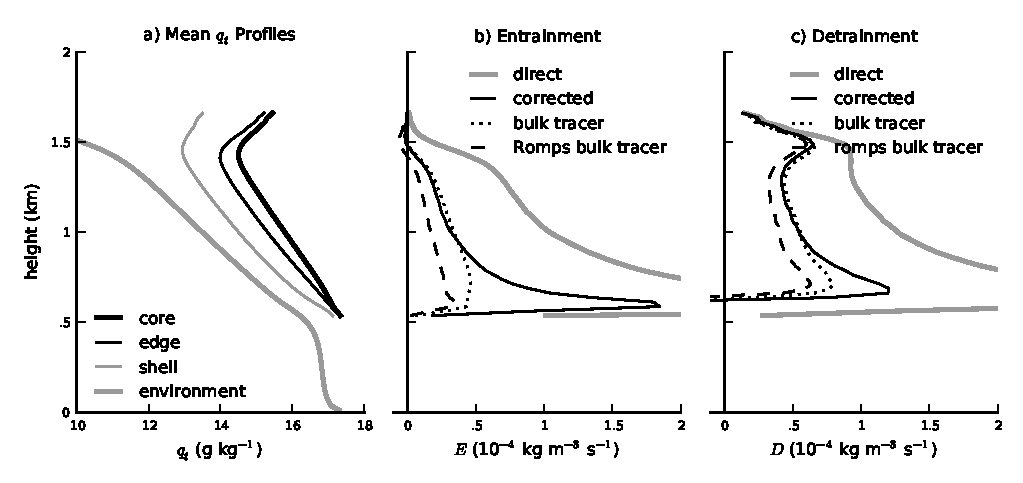
\includegraphics[width=39pc]{./figures/shell_correction}
  \caption{Result of correcting direct entrainment values for the presence of 
  the moist cloud shell.  a) Mean profiles of total specific water in the 
  cloud core (thick black line), cloud core edge (thin black line), cloud core 
  shell (thin grey line), and cloud core environemnt (thick grey line).  These 
  total specific water values are used to correct values of b) entrainment and 
  c) detrainment; shown are the direct flux calculation of \cite{Romps2010}
  (thick grey line), the bulk tracer budget calculation of \cite{Siebesma1995} 
  (thin grey line), and the direct flux calculation corrected by the mean 
  core shell and edge values (black line).
  }
  \label{fig:shell_correction}
\end{figure}

\begin{figure}
  \label{fig:Reynolds_correction}
  \noindent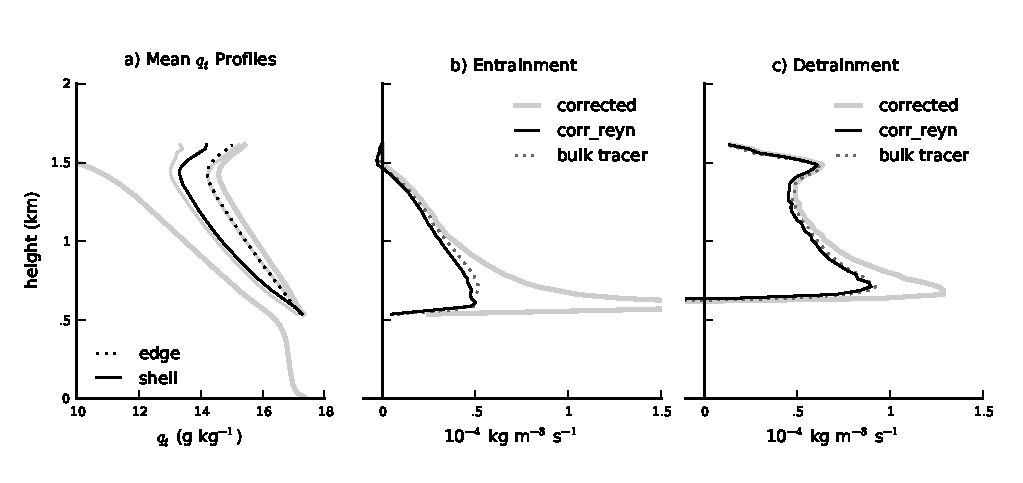
\includegraphics[width=39pc]{./figures/reynolds_correction}
  \caption{Result of correcting direct entrainment values by the effective 
  entrainment and detrainment total specific water values, which include the 
  effects of Reynolds correlations between mass fluxes and humidity values.
  a) Mean profiles of the effective total specific water value for 
  the entrainment (black line) and detrainment (dotted line), overlaid on the 
  mean core, edge, shell, and environment profiles (grey line).  These 
  values are used to correct values of b) entrainment and c) detrainment; shown 
  are the direct flux calculation of \cite{Romps2010} corrected by the mean 
  core shell and edge values (thick grey line), the bulk tracer budget 
  calculation of \cite{Siebesma1995} (thin grey line), and the direct flux 
  calculation corrected by the effective core shell and edge values (black 
  line).}
\end{figure}

\begin{figure}
  \label{fig:numerical_correction}
  \noindent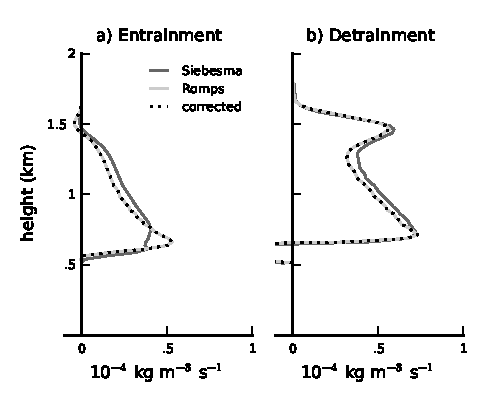
\includegraphics[width=20pc]{./figures/numerical_correction}
  \caption{Comparison of specific humidity a) entrainment and b) detrainment 
  values calculated via the methods in \cite{Siebesma1995} (black line) and 
  \cite{Romps2010} (grey line), and the direct flux calculation of Romps 
  corrected by the effective entrainment and detrainment specific humidities
  (dotted line).
  }
\end{figure}

% ONE-COLUMN figure/table, including eps graphics
%
% \begin{figure}
% \noindent\includegraphics[width=20pc]{samplefigure.eps}
% \caption{Caption text here}
% \end{figure}
% \end{document}
%
% \begin{table}
% \caption{}
% \end{table}
%
% ---------------
% TWO-COLUMN figure/table
%
% \begin{figure*}
% \noindent\includegraphics[width=39pc]{samplefigure.eps}
% \caption{Caption text here}
% \end{figure*}
%
% \begin{table*}
% \caption{Caption text here}
% \end{table*}
%
% see below for how to make landscape figures or tables

%%% End the article here:

\end{document}

%%%%%%%%%%%%%%%%%%%%%%%%%%%%%%%%%%%%%%%%%%%%%%%%%%%%%%%%%%%%%%%


%% ------------------------------------------------------------------------ %%
%
%  IN-TEXT LISTS
%
%% ------------------------------------------------------------------------ %%

% Do not use bulleted lists; enumerated lists are okay.
% \begin{enumerate}
% \item
% \item
% \item
% \end{enumerate}

%% ------------------------------------------------------------------------ %%
%
%  EQUATIONS
%
%% ------------------------------------------------------------------------ %%

% Single-line equations are centered.

% Math coded inside display math mode \[ ...\]
% will not be numbered e.g.:
% \[ x^2=y^2 + z^2\]

% Math coded inside \begin{equation} and \end{equation} will
% be automatically numbered e.g.:
% \begin{equation}
% x^2=y^2 + z^2
% \end{equation}

% IF YOU HAVE MULTI-LINE EQUATIONS, PLEASE
% BREAK THE EQUATIONS INTO TWO OR MORE LINES
% OF SINGLE COLUMN WIDTH (20 pc, 8.3 cm)
% using double backslashes (\\).

% To create multiline equations, use the
% \begin{eqnarray} and \end{eqnarray} environment
% as demonstrated below.
\begin{eqnarray}
  x_{1} & = & (x - x_{0}) \cos \Theta \nonumber \\
        && + (y - y_{0}) \sin \Theta  \nonumber \\
  y_{1} & = & -(x - x_{0}) \sin \Theta \nonumber \\
        && + (y - y_{0}) \cos \Theta.
\end{eqnarray}

If you don't want an equation number, use the star form:
\begin{eqnarray*}...\end{eqnarray*}

% Break each line at a sign of operation
% (+, -, etc.) if possible, with the sign of operation
% on the new line.

% Indent second and subsequent lines to align with
% the first character following the equal sign on the
% first line.

% Use an \hspace{} command to insert horizontal space
% into your equation if necessary. Place an appropriate
% unit of measure between the curly braces, e.g.
% \hspace{1in}; you may have to experiment to achieve
% the correct amount of space.

% There is another multiline equation environment:
% \begin{aguleftmath}...\end{aguleftmath}
% The equation is aligned left and the second line indents to
% the width of a paragraph indent (AGU style)


%% ------------------------------------------------------------------------ %%
%
%  EQUATION NUMBERING: COUNTER
%
%% ------------------------------------------------------------------------ %%

% You may change equation numbering by resetting
% the equation counter or by explicitly numbering
% an equation.

% To explicitly number an equation, type \eqnum{}
% (with the desired number between the brackets)
% after the \begin{equation} or \begin{eqnarray}
% command.  The \eqnum{} command will affect only
% the equation it appears with; LaTeX will number
% any equations appearing later in the manuscript
% according to the equation counter.
%
% To reset the equation counter, place the setcounter{equation}
% command in front of your equation(s).
%\setcounter{equation}{0}

% Set the equation counter to 0 if the next
% number needed is 1 or set it to 7 if the
% next number needed is 8, etc.
%
% The \setcounter{equation} command does affect
% equations appearing later in the manuscript.

% If you have a multiline equation that needs only
% one equation number, use a \nonumber command in
% front of the double backslashes (\\) as shown in
% the multiline equation above.



%%%%%%%%%%%%%%%%%%%%%%%%%%%%%%%%%%%%%%%%%%%%%%%%%%%%%%
%% Landscape figure and table examples
%
% ---------------
% Landscape (broadside) figure/table
% (These objects will not display properly in draft mode, use galley.)
%
% ONE-COLUMN landscape figure and table
%
% \begin{landscapefigure}
% \includegraphics[height=.75\mycolumnwidth,width=42pc]{samplefigure.eps}
% \caption{Caption text here}
% \end{landscapefigure}
%
% \begin{landscapetable}
% \caption{Caption text here}
% \begin{tabular*}{\hsize}{@{\extracolsep{\fill}}lcccc}
% \tableline
% ....
% \tableline\\
% \multicolumn5l{(a) Algorithms from Numerical Recipes}\\
% \end{tabular*}
% \tablenotetext{}{}
% \tablecomments{}
% \end{landscapetable}
%
% FULL-PAGE landscape figures and tables
%
% \begin{figure*}[p]
% \begin{landscapefigure*}
% illustration here
% \caption{caption here}
% \end{landscapefigure*}
% \end{figure*}
%
% \begin{table}[p]
% \begin{landscapetable*}
% \caption{}
% \begin{tabular*}{\textheight}{@{\extracolsep{\fill}}lccrrrcrrr}
% ....
% \end{tabular*}
% \begin{tablenotes}
% ...
% \end{tablenotes}
% \end{landscapetable*}
% \end{table}
%
